\section{Mollification of sets of least perimeter}\label{MollifierSection}
In this section our goal is to show that given a set $U$ of least perimeter, we can find a $C^1$ hypersurface $N$ which approximates $\partial^* U$ arbitrarily well.

\begin{proposition}\label{mollifier quant}
    For every $P \in M$ and every $\varepsilon > 0$, there exists $\gamma^* > 0$ such that $P \mapsto \gamma^*$ is continuous and such that for every $\delta > 0$ such that $\exp_P: \{v: g(v, v) < \delta\} \to M$ is injective, all vector fields $X, Y$ with $1/2 \leq g(X, X), g(Y, Y) \leq 2$ and every set $U$ of least perimeter, $u = 1_U$, such that
    \begin{equation}\label{bootstrap the mollifier}
    \gamma = \delta^{1 - d}\int_{B(P, \delta)} |du| - Xu ~\vol < \gamma^*:
    \end{equation}

    For every almost every $t \in (0, \delta)$, there exists a set $V$ of $C^1$ perimeter in $B(P, t)$, $v = 1_V$, such that
    \begin{align}
    |V \cap B(P, t)| &\leq \eta(V, B(P, t)) + \varepsilon \delta^{d - 1} \gamma, \label{mollifier quant1}\\
    \left|\int_{B(P, t)} |du| - |dv| ~\vol\right| &\leq \varepsilon \delta^{d - 1} \gamma, \label{mollifier quant2}\\
    \left|\int_{B(P, t)} Y(u - v) ~\vol\right| &\leq \varepsilon \delta^{d - 1} \gamma, \label{mollifier quant3}\\
    (\normal_V, X) &\geq (1 - \varepsilon) g(X, X) \text{ on } B_{t-\varepsilon}. \label{mollifier quant4}
    \end{align}
    Moreover, $V$ does not depend on $Y$.
\end{proposition}

The euclidean analogue of this proposition is \cite[Lemma 5.5]{Miranda66}.
For an exposition of the euclidean proof, we recommend \cite[Chapter 7]{Giusti77}.
We use the same integral kernel as \cite[Chapter 7]{Giusti77}, and much of our argument is the same, but we must take care to control the error terms arising from $\Ric_g$.

We proceed using compactness and contradiction. More precisely, suppose that the following lemma is true:

\begin{lemma}\label{mollifier proposition}
Let $(U_n)$ be a sequence of sets with indicator functions $u_n$, let $X, Y$ be vector fields with $1/2 \leq g(X, X), g(Y, Y) \leq 2$, and let
$$\gamma_n = \int_{B(P, 1)} |du_n| - Xu_n ~\vol.$$
Suppose that in addition:
\begin{enumerate}
\item $(u_n)$ has least gradient.
\item $(\gamma_n) \in \ell^1$.
\item The exponential map $\exp_P$ is injective on $\{v \in T_PM: g(v, v) < 1\}$.
\end{enumerate}

Then for almost every $t \in (0, 1)$ there exist open sets $V_n$ with $C^1$ boundary and indicator $v_n$, such that for every $j \in \{0, \dots, d - 1\}$,
\begin{align}
|\partial V_n \cap B_t| &\leq \eta(V_n, B_t) + o(\gamma_n), \label{mollifier prop1}\\
\left|\int_{B_t} |du_n| - |dv_n| ~\vol\right| &\ll \gamma_n, \label{mollifier prop2}\\
\left|\int_{B_t} Y(u_n - v_n)~\vol\right| &\lesssim \gamma_n^2, \label{mollifier prop3}\\
\lim_{n \to \infty} g(\normal_{L_n}, X) &= g(X, X), \label{mollifier prop4}
\end{align}
and the limit in (\ref{mollifier prop4}) is locally uniform.
\end{lemma}

By rescaling $g$ appropriately, we may assume that $\delta \geq 1$.
Then if the claim is not true, there exist $P \in M, \varepsilon > 0, X, Y$, and $\gamma_n \to 0$, such that there is a set $U_n$ of least perimeter satisfying (\ref{bootstrap the mollifier}) with $U = U_n$, $\gamma = \gamma_n$, and an exceptional set $T_n \subseteq (0, 1)$ of positive measure such that for every $t \in T_n$ and every set $V$ of $C^1$ perimeter in $B(P, t)$, one of (\ref{mollifier quant1}, \ref{mollifier quant2}, \ref{mollifier quant3}, \ref{mollifier quant4}) is false.
After passing to a subsequence we may assume that $(\gamma_n) \in \ell^1$.
If we take $V = V_n$ where $V_n$ is given by Lemma \ref{mollifier proposition}, the failure of the conjunction of (\ref{mollifier quant1}, \ref{mollifier quant2}, \ref{mollifier quant3}, \ref{mollifier quant4}) contradicts the conjunction of (\ref{mollifier prop1}, \ref{mollifier prop2}, \ref{mollifier prop3}, \ref{mollifier prop4}), which completes the proof of Proposition \ref{mollifier quant}.
So it suffices to show Lemma \ref{mollifier proposition}.

%%%%%%%%%%%%%%%%%%%%%%%%%%%%%%%%%%%%%%%%%%%%%%%%%%%%%%%

\subsection{Polar coordinates}
Suppose that we are in the situation of Lemma \ref{mollifier proposition}, namely we are given a point $P \in M$ such that the exponential map is a diffeomorphism
\begin{equation}\label{exp map mollify}
\exp_P: \{v \in T_PM: g(v, v) < 1\} \to B_1.
\end{equation}
Then we may introduce polar coordinates
\begin{equation}\label{polar coordinates mollify}
(r, \Theta): B_1 \setminus \{P\} \to (0, 1) \times \Sph^{d - 1},
\end{equation}
where $\Theta = (\theta_1, \dots, \theta_{d - 1})$,
for which $g(\partial_r, \partial_{\theta_i}) = 0$ and $g(\partial_r, \partial_r) = 1$.
We also define
$$\kappa = -\frac{R(P)|\Sph^{d - 1}|}{6d}$$
where $R$ is the scalar curvature field of $g$.
With this notation we have
\begin{equation}\label{area of sphere form}
|\partial B_\rho| = |\Sph^{d - 1}|\rho^{d - 1} + \kappa \rho^{d + 1} + O(\rho^{d + 3}),
\end{equation}
and $\kappa$ and the above implied constant depend continuously on $P$; see \cite{gray1974volume} for a proof.
We use this fact to estimate the normal vector of a set of least perimeter, as follows.

\begin{lemma}\label{scalar curvature monotonicity}
If $r_1 < r_2$, $U$ is a set of least perimeter, $u = 1_U$, and $Q \in \partial^* U$,
$$r_2^{1 - d}\int_{B(Q, r_2)} Xu ~\vol - r_1^{1 - d}|\partial^* U \cap B(Q, r_1)| \leq (r_2^2 - r_1^2)\kappa(Q) + O(r_2^4).$$
\end{lemma}
\begin{proof}
Since $U$ is a set of least perimeter, in particular its reduced boundary in $B(Q, r_1)$ has less area than $\partial B(Q, r_1)$.
By the fundamental theorem of calculus and the Cauchy-Schwarz inequality,
$$\int_{B(Q, r_2)} Xu ~\vol = \int_{\partial B(Q, r_2) \cap U} g(\normal_{\partial B(Q, r_2)}, X) ~\vol \leq \int_{\partial B(Q, r_2) \cap U} \vol = |\partial B(Q, r_2)|.$$
Applying (\ref{area of sphere form}),
\begin{align*}
r_2^{1 - d}|\partial B(Q, r_2)| - r_1^{1 - d}|\partial^* U \cap B(Q, r_1)|
&\leq r_2^{1 - d}|\partial B(Q, r_2)| - r_1^{1 - d}|\partial B(Q, r_1)| \\
&\leq |\Sph^{d - 1}| + r_2^2\kappa(Q) + O(r_2^4) - |\Sph^{d - 1}| - r_1^2 \kappa(Q) + O(r_1^4)\\
&\leq (r_2^2 - r_1^2)\kappa(Q) + O(r_2^4).\qedhere
\end{align*}
\end{proof}

We now construct the integral kernel that we will use in the proof of Lemma \ref{mollifier proposition}.
Using the identification (\ref{exp map mollify}), we can define the difference of two points in $B_1$ and so can define the convolution $\omega * u$ of a function $u \in L^1_l(B_1)$ with any volume form $\omega$ with compact support in $B_1$.

\begin{definition}
Define the volume form
$$\chi_\varepsilon = \frac{r^{d - 1}}{\varepsilon^d}\left(1 - \frac{r}{\varepsilon}\right)1_{r < \varepsilon} ~dr \wedge d\mu(\Theta)$$
where $\mu$ is the usual measure on $\Sph^{d - 1}$, but normalized so that $\mu(\Sph^{d - 1}) = d(d + 1)$.
For a function $u \in L^1_l$, we define $u_\varepsilon = \chi_\varepsilon * u$.
\end{definition}

The integration kernel $\chi_\varepsilon$ was introduced in \cite[Chapter 7]{Giusti77} in order to mollify sets of least perimeter on euclidean space.
The point is that, for the purposes of our later arguments, we will only need $u_\varepsilon \in C^1$, and so we can use a Lipschitz kernel which satisfies certain convenient estimates \cite[Lemmata 7.1--7.2]{Giusti77}.
Our purpose is now to prove an analogue of such estimates in our setting, but before we do so, we record the basic properties of $\chi_\varepsilon$:

\begin{lemma}\label{mollifier props}
$\chi_\varepsilon$ has the following properties:
\begin{enumerate}
\item $\chi_\varepsilon$ is supported on $B_\varepsilon$.
\item The Radon-Nikod\'ym derivative $F = \chi_\varepsilon/\vol$ is Lipschitz continuous and has the Taylor expansion
\begin{equation}\label{RN mollify}
F(r, \Theta) = \frac{d(d + 1)}{\varepsilon^d} \left(1 - \frac{r}{\varepsilon}\right) 1_{r < \varepsilon}(1 - \kappa r^2 + O(r^4)).
\end{equation}
\item If $u$ is an indicator function then $(du_\varepsilon) = (du)_\varepsilon$ is a continuous $1$-form.
\item $\chi_\varepsilon$ converges in the weakstar topology to the Dirac measure at $Q$.
\item On $B_\varepsilon \setminus \{P\}$, $\partial_{\theta_i} F = 0$ and $\partial_r F = O(r)$.
\item For every $Q \in B_1$, $\delta > 0$, $x \in B_1$, and $y \in B(Q, \delta)$,
\begin{equation}\label{approximation of mollifier 2}
F(x - y) \sim \frac{1}{\varepsilon^d}\left(1 - \frac{d(x, Q)}{\varepsilon}\right)
\end{equation}
where the implied constant remains bounded as $\varepsilon,\delta \to 0$.
\end{enumerate}
\end{lemma}
\begin{proof}
These assertions follow from the definitions and (\ref{area of sphere form}).
\end{proof}

\begin{lemma}\label{Giusti71}
There exists $c > 0$ such that for every indicator function $u = 1_U$, if
$$c\varepsilon^2 + c\rho^2 \leq u_\varepsilon(x) \leq 1 - c\varepsilon^2 - c\rho^2,$$
then
\begin{equation}\label{Giusti71 claim}
d(x, \partial U) < \varepsilon(1 - \rho).
\end{equation}
\end{lemma}
\begin{proof}
Suppose that (\ref{Giusti71 claim}) fails for some $x \in M$. Then either $d(x, U) \geq \varepsilon(1 - \rho)$ or $d(x, M \setminus U) \geq \varepsilon(1 - \rho)$.
We estimate $\omega(y) = u(y)\chi_\varepsilon(x - y)$ on the annulus $A = B(x, \varepsilon) \setminus B(x, \varepsilon(1 - \rho))$ using (\ref{RN mollify}) and Taylor's theorem, as follows:
\begin{align*}
\int_A \omega &= \int_A F ~\vol \\
&= \frac{d(d + 1)}{\varepsilon^d} \int_{\varepsilon(1 - \rho)}^\varepsilon r^{d - 1}\left(1 - \frac{r}{\varepsilon}\right)(1 + O(r^2)) ~dr \\
&= \frac{d(d + 1)}{\varepsilon^d} \int_{\varepsilon(1 - \rho)}^\varepsilon r^{d - 1} - \frac{r^d}{\varepsilon} + O(r^{d + 1}) ~dr\\
&= \frac{d(d + 1)}{\varepsilon^d} \left[\frac{\varepsilon^d}{d}(1 - (1 - \rho)^d) - \frac{\varepsilon^d}{d + 1}(1 - (1 - \rho)^{d + 1}) + O(\varepsilon^{d + 2})\right]\\
&= 1 - (d + 1)(1 - d\rho + O(\rho^2)) + d(1 - (d + 1)\rho + O(\rho^2)) + O(\varepsilon^2) \\
&= O(\rho^2 + \varepsilon^2).
\end{align*}
If $d(x, U) \geq \varepsilon(1 - \rho)$, then $u\omega$ is supported inside $A$, thus $u_\varepsilon(x) \gtrsim \rho^2 + \varepsilon^2$.
Conversely, if $d(x, M \setminus U) \geq \varepsilon(1 - \rho)$, then $(1 - u)\omega$ is supported inside $A$, thus $1 - u_\varepsilon(x) \lesssim \rho^2 + \varepsilon^2$.
\end{proof}

\begin{lemma}\label{Giusti72}
Let $u \in BV(B_1)$ and $\tau, \varepsilon > 0$. If $\tau + \varepsilon \leq 1$, then
$$\int_{B_\tau} |u_\varepsilon - u| ~\vol \lesssim \varepsilon \int_{B_{\tau + \varepsilon}} |du| ~\vol$$
$$\int_{B_\tau} |du_\varepsilon| - |du| ~\vol \lesssim \int_{B_{\tau + \varepsilon} \setminus B_\tau} |du| ~\vol.$$
\end{lemma}
\begin{proof}
If we suppose that
$$c^{-1} \vol^{\mathrm{euc}} \leq \vol \leq c\vol^{\mathrm{euc}}$$
where $\vol^{\mathrm{euc}}$ is the pushforward by $\exp_P$ of the euclidean volume form on $T_PM$ (as given by (\ref{exp map mollify})), then the assertions are immediate from \cite[Lemma 7.2]{Giusti77} with implied constant $c^2$.
Such a constant $c > 0$ must exist, since $\sqrt{\det g}$ is bounded on the compact set $B_1$.
\end{proof}

%%%%%%%%%%%%%%%%%%%%%%%%%%%%%%%%%%%%%%%%%%%%%%%%%%%%%%

\subsection{\texorpdfstring{$C^1$}{C1} level sets}
The main step in the proof of Lemma \ref{mollifier proposition} is to generalize \cite[Theorem 7.3, Remark 7.4]{Giusti77}:

\begin{lemma}\label{main mollifier lemma}
Let $\gamma, p > 0$, let $U$ be a set of least perimeter, $u = 1_U$, and suppose that
\begin{equation}\label{hypothesis on main mollifier lemma}
\int_{B_1} (|du| - Xu) ~\vol \leq \gamma.
\end{equation}
Let $\varepsilon = \gamma^p$, $\sigma = \gamma^{1/(2(d - 1))}$, and $\varphi = u_\varepsilon$. Then there exists $c > 0$ such that
\begin{equation}\label{claim on main mollifier lemma}
\inf_{\substack{r < \sigma\\\varphi \in (c\gamma^2, 1 - c\gamma^2)}} \frac{X \varphi}{|d\varphi|} > 1 - O(\gamma^{O(1)})
\end{equation}
and for every $y \in (c\gamma^2, 1 - c\gamma^2)$ the level set $\partial \{\varphi > y\} \cap \{r < \sigma\}$ is a $C^1$ hypersurface.
\end{lemma}

The proof of Lemma \ref{main mollifier lemma} is analogous to the proof of \cite[Theorem 7.3]{Giusti77}, using the results of \S\ref{LeastGradientFunctions} as a substitute for \cite[Chapter 5]{Giusti77}.
Here is the main idea: $|du| ~\vol$ is a Radon measure of Ahlfors-David dimension $d - 1$ (c.f. Proposition \ref{doubling dimension}), so we may cover the domain of integration with open sets of volume $\sim \delta^d\varepsilon^d$ where $\delta > 0$ is a small parameter that determines the cardinality of the cover.
Then $|du| - Xu ~\vol$ assigns a slightly shrunken version of each such set a measure $\sim \delta^{d - 1} \varepsilon^{d - 1}$, while $|du|~\vol$ assigns the set in the cover a comparable measure, by the monotonicity formula, Proposition \ref{Monotonicity Formula}.
Thus $|du| - Xu ~\vol$ is controlled by $|du|~\vol$.

\begin{proof}[Proof of Lemma \ref{main mollifier lemma}, assuming (\ref{bound on balls}, \ref{bound on balls 2})]
Let $\delta = \gamma^d > 0$ and select disjoint balls $V_1, \dots, V_N$, centered on $Q_n$, in $\partial^* U \cap B_{\varepsilon(1 - 2\delta)}$ of radius $\delta\varepsilon$ so that the dilates $2V_n$ cover $\partial^* U \cap B_{\varepsilon(1 - 2\delta)}$.
It is easy to show that such a cover exists, because $\overline{\partial^* U \cap B_{\varepsilon(1 - 2\delta)}}$ is compact if $\gamma$ is small enough, so for such a $\gamma$ we can greedily select $Q_n \in \overline{\partial^* U \cap B_{\varepsilon(1 - 2\delta)}}$ to maximize $\min(d(Q_1, Q_n), \dots, d(Q_{n - 1}, Q_n))$.
We set $V_0 = B_\varepsilon \setminus B_{\varepsilon(1 - 2\delta)}$.

\begin{figure}[ht]
\caption{The sets $V_0, \dots, V_n$ (in dark grey) are an annulus and several small balls of radius $\delta$, which approximately cover the boundary of the set $U$ (in light grey).}
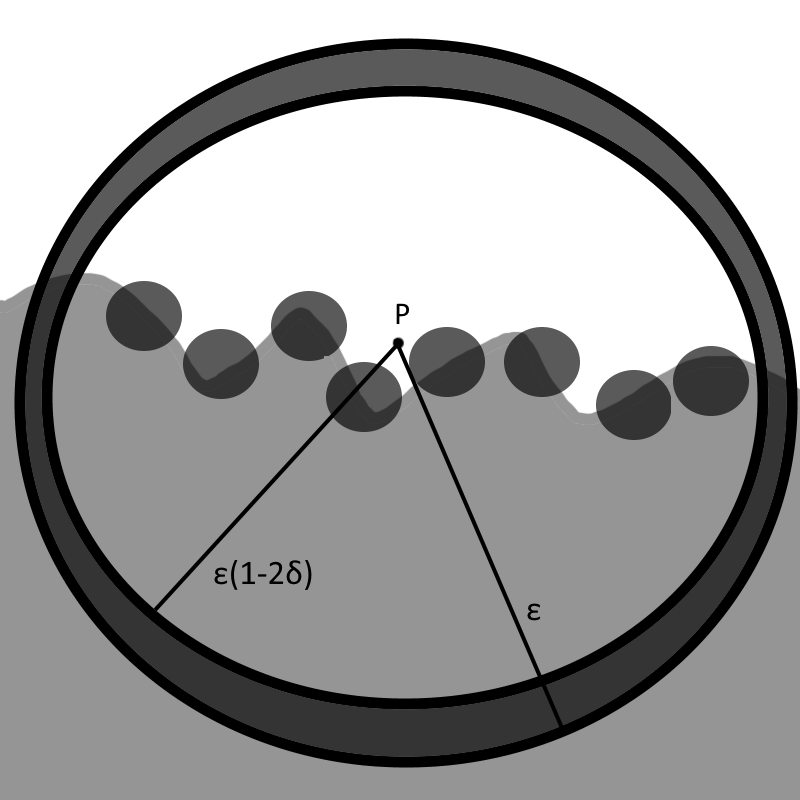
\includegraphics[width=0.4\textwidth]{covering lemma}
\end{figure}

Since $du$ is supported in $\bigcup_n 2V_n$,
$$|d\varphi|(x) - X\varphi(x) = \int_{B_\varepsilon} \chi_\varepsilon(x - \cdot)(|du| - Xu) \leq \sum_{n=0}^N \int_{2V_n} \chi_\varepsilon(x - \cdot)(|du| - Xu).$$
So, we shall show
\begin{equation}\label{bound on balls}
\int_{2V_n} \chi_\varepsilon(x - \cdot)(|du| - Xu) \lesssim_{g, p, P} \gamma^{O(1)} \int_{V_n} \chi_\varepsilon(x - \cdot)|du|
\end{equation}
for $n \geq 1$ and
\begin{equation}\label{bound on balls 2}
\int_{V_0} \chi_\varepsilon(x - \cdot)(|du| - Xu) \lesssim_{g, p, P} \gamma^{O(1)} \int_{B_\varepsilon} \chi_\varepsilon(x - \cdot)|du|,
\end{equation}
provided that $x = (r, \Theta)$ satisfies $r < \sigma$ and $\varphi \in (o(\gamma), 1 - o(\gamma))$.
If (\ref{bound on balls}, \ref{bound on balls 2}) are true, then since the balls $V_n$ are disjoint, we can sum over $n$ to obtain
\begin{equation}\label{claim on main mollifier lemma 2}|d\varphi|(x) - X\varphi(x) \lesssim_{g, p, P} \gamma^{O(1)} \int_{B_\varepsilon} \chi_\varepsilon(x - \cdot)|du| \leq \gamma^{O(1)} |d\varphi|(x),
\end{equation}
which implies (\ref{claim on main mollifier lemma}). Thus we may fix
$$x \in \partial^* U \cap \{r < \sigma\} \cap \{\varphi \in (f(\gamma), 1 - f(\gamma)),$$
and choose $\gamma$ so small that (\ref{claim on main mollifier lemma 2}) simplifies to $X\varphi(x) \gtrsim |d\varphi(x)|$.
Thus, in particular,
$$X\varphi(x) \gtrsim \int_{B_\varepsilon} \chi_\varepsilon(x - \cdot) |du| > 0.$$
By Lemma \ref{mollifier props}, $d\varphi$ is continuous, so the level sets of $\varphi$ must be $C^1$.
\end{proof}

\begin{proof}[Proof of (\ref{bound on balls})]
By (\ref{approximation of mollifier 2}), if $\gamma$ is small enough depending on $g$\footnote{One might worry that we frequently rescale $g$ in this paper.
However, in all of our rescalings, the curvature tensor remains in some bounded set, so these rescalings will never send $\gamma$ to $0$.}, then for every $y \in 2V_n$,
\begin{align*}
\int_{2V_n} \chi_\varepsilon(x - \cdot)(|du| - Xu) &\lesssim F_n(x) \int_{2V_n} |du| - Xu ~\vol, \\
F_n(x) &:= \frac{1}{\varepsilon^d}\left(1 - \frac{d(x, Q_n)}{\varepsilon}\right).
\end{align*}
If $\gamma$ is chosen small enough, then $\sigma > 2\delta\varepsilon$ and so if we set $W_n = B(Q_n, \sigma)$ and apply Proposition \ref{Monotonicity Formula},
\begin{align*}
\int_{2V_n}|du| - Xu ~\vol &\leq
B \left[\sigma^{1 - d}\int_{W_n} |du| - Xu ~\vol + \sigma^{1 - d}\int_{W_n} Xu ~\vol - (2\delta\varepsilon)^{1 - d}\int_{2V_n} Xu ~\vol \right],\\
B &:= e^{O(1)(\sigma^2 - 4\delta^2\varepsilon^2)}(2\delta\varepsilon)^{d - 1}.
\end{align*}
From Taylor's theorem and the fact that $\sigma > 2\delta\varepsilon$,
\begin{align*}
B \lesssim \delta^{d - 1} \varepsilon^{d - 1} + \sigma^2 \delta^{d - 1} \varepsilon^{d - 1} \lesssim \delta^{d - 1} \varepsilon^{d - 1}
\end{align*}
if $\gamma$ is small.
By (\ref{hypothesis on main mollifier lemma}),
$$\sigma^{1 - d}\int_{W_n} |du| - Xu ~\vol \leq \gamma^{\frac{1 - d}{2(d - 1)} + 1} = \gamma^{1/2}.$$
By Proposition \ref{Monotonicity Formula},
\begin{align*}
\sigma^{1 - d}\int_{W_n} Xu ~\vol - (2\delta\varepsilon)^{1 - d}\int_{2V_n} Xu ~\vol &\lesssim (1 + \alpha)\sqrt{\sigma^{1 - d} \int_{W_n} |du| ~\vol - (2\delta\varepsilon)^{1 - d} \int_{2V_n} |du| ~\vol},\\
&\alpha := (d - 1)\log \frac{\sigma}{2\delta\varepsilon}.
\end{align*}
By Lemma \ref{scalar curvature monotonicity},
$$\sigma^{1 - d} \int_{W_n} X u ~\vol - (2\delta\varepsilon)^{1 - d} \int_{2V_n} |du| ~\vol \leq (\sigma^2 -4\delta^2\varepsilon^2) \kappa(Q_n) + O(\sigma^4) \lesssim \sigma^2,$$
so by (\ref{hypothesis on main mollifier lemma}),
\begin{align*}
\sigma^{1 - d} \int_{W_n} |du| ~\vol - (2\delta\varepsilon)^{1 - d} \int_{2V_n} |du| ~\vol &= \sigma^{1 - d} \int_{W_n} |du| - Xu ~\vol \\
&\qquad + \sigma^{1 - d} \int_{W_n} Xu ~\vol - (2\delta\varepsilon)^{d - 1} \int_{W_n} |du| ~\vol \\
&\leq \gamma + O(\sigma^2) \lesssim \sigma^2.
\end{align*}
It follows from the definitions that
$$(1 + \alpha)\sigma \lesssim -\gamma^{1/2(d - 1)} \log \gamma \lesssim \gamma^{1/3(d - 1)}.$$
Summing up everything in this step of the proof thus far,
\begin{equation}\label{big bound 1}
\int_{2V_n} \chi_\varepsilon(x - \cdot)(|du| - Xu) ~\vol \lesssim \delta^{d - 1} \varepsilon^{d - 1} F_n(x) \gamma^{1/3(d - 1)}.
\end{equation}
Since $U$ has least perimeter, Proposition \ref{doubling dimension} implies that
$$\delta^{d - 1} \varepsilon^{d - 1} \lesssim \int_{V_n} |du| ~\vol,$$
so by (\ref{approximation of mollifier 2}, \ref{big bound 1}),
\begin{align*}
\int_{2V_n} \chi_\varepsilon(x - \cdot)(|du| - Xu) ~\vol
&\lesssim \gamma^{1/3(d - 1)} \int_{V_n} \chi_\varepsilon(x - \cdot)|du|.
\qedhere \end{align*}
\end{proof}

\begin{proof}[Proof of (\ref{bound on balls 2})]
From (\ref{approximation of mollifier 2}) it easily follows that for $y \in V_0$, $\chi_\varepsilon(x - y)/\vol(x - y) \lesssim \frac{\delta}{\varepsilon^d}$,
whence, by minimality of $\partial^* U$,
\begin{align*}
\int_{V_0} \chi_\varepsilon(x - \cdot)(|du| - Xu) &\lesssim \frac{\delta}{\varepsilon^d} \int_{B_\varepsilon} |du| ~\vol \lesssim \frac{\delta}{\varepsilon^d} |\partial B_\varepsilon| \lesssim \frac{\delta}{\varepsilon}.
\end{align*}
By Lemma \ref{Giusti71}, there exists $c > 0$ such that if $\varphi \in (c\gamma^2, 1 - c\gamma^2)$, then $d(x, \partial U) < \varepsilon(1 - \gamma)$, so in particular we can find $Q \in \partial^* U$ such that $d(x, Q) < \varepsilon(1 - \gamma)$.
If $d(y, Q) < \gamma\varepsilon/2$, then
$$d(x, y) \leq \varepsilon - \gamma\varepsilon + \frac{\gamma\varepsilon}{2} \leq \varepsilon - \frac{\gamma\varepsilon}{2},$$
so by (\ref{approximation of mollifier 2}), $\chi_\varepsilon(x - y)/\vol(x - y) \gtrsim \frac{\gamma}{\varepsilon^d}$
for every $y \in B(Q, \gamma\varepsilon/2)$.
In particular, since $\delta = \gamma^d$, minimality of $\partial^* U$ gives
\begin{align*}
\int_{V_0} \chi_\varepsilon(x - \cdot)(|du| - Xu) &\lesssim \frac{\delta}{\gamma^{d - 1}} \frac{\gamma^{d - 1}}{\varepsilon}\\
&\lesssim \gamma |\partial B(Q, \gamma\varepsilon/2)| \int_{B(Q, \gamma\varepsilon/2)} \chi_\varepsilon(x - \cdot) \\
&\lesssim \gamma \int_{B(Q, \gamma\varepsilon/2)} \chi_\varepsilon(x - \cdot) |du|\\
&\lesssim \gamma \int_{B_\varepsilon} \chi_\varepsilon(x - \cdot) |du|. \qedhere
\end{align*}
\end{proof}

%%%%%%%%%%%%%%%%%%%%%%%%%%%%%%%%%%%%%%%%%%%%%%%%%%%%%

\subsection{The qualitative case}
We now complete the proof of Lemma \ref{mollifier proposition}.
Select $t \in (0, 1)$ uniformly at random.
Let $w_n = (u_n)_{\gamma_n^4}$, let $c$ be the constant given by Lemma \ref{main mollifier lemma}, and let $a_n = c\gamma_n$, $b_n = 1 - c\gamma_n$.
0By Proposition \ref{Coarea2},
$$\int_{B_t} |dw_n| ~\vol = \int_0^1 |\partial^* \{w_n > y\} \cap B_t| ~dy \geq \int_{a_n}^{b_n} |\partial^* \{w_n > y\} \cap B_t| ~dy.$$
By the mean value theorem, there exists $y_n \in (a_n, b_n)$ such that
\begin{equation}\label{MVT mollifier}
|\partial^* \{w_n > y_n\} \cap B_t| \leq \frac{1}{b_n - a_n} \int_{B_t} |dw_n| ~\vol.
\end{equation}
If set $V_n = \{w_n > y_n\}$, $v_n = 1_{V_n}$, then $V_n$ has $C^1$ boundary in $B_t$ by definition of $a_n, b_n$, and from (\ref{claim on main mollifier lemma}), the locally uniform convergence (\ref{mollifier prop4}) holds.

So it remains to show that (\ref{mollifier prop1}--\ref{mollifier prop3}) hold almost surely.
Towards this end we will later show that
\begin{align}
|\partial V_n \cap B_t| &\leq |\partial^* U_n \cap B_t| + o(\gamma_n), \label{approximation of surface area} \\
\int_{\partial B_t} |u_n - v_n| ~\vol_{\partial B_t} &\lesssim \gamma_n^2. \label{approximation of volume}
\end{align}
If (\ref{approximation of surface area}, \ref{approximation of volume}) are true,
then by (\ref{a priori estimate 3}, \ref{approximation of volume}),
$$|\partial^* U_n \cap B_t| \leq |\partial V_n \cap B_t| + o(\gamma_n)$$
so by (\ref{approximation of surface area}), (\ref{mollifier prop2}) holds.
From an integration by parts using the estimate $1/2 \leq g(Y, Y) \leq 2$, and (\ref{approximation of volume}),
\begin{align*}
\left|\int_\Omega Y(u_j - v_j) ~\vol\right|
&\leq \left|\int_{\partial \Omega} (u_j - v_j)g(Y, \normal) ~\vol_{\partial \Omega}\right| \\
&\lesssim \int_{\partial \Omega} |u_j - v_j| ~\vol_{\partial \Omega} \lesssim \gamma_n^2
\end{align*}
which gives (\ref{mollifier prop3}).
By the fact that $U_n$ has least perimeter, and (\ref{a priori estimate 1}, \ref{mollifier prop2}),
\begin{align*}
|\partial V_n \cap B_t| &\leq |\partial U_n \cap B_t| + o(\gamma_n) \\
&= \eta(U_n, B_t) + o(\gamma_n)\\
&\leq \eta(V_n, B_t) + \int_{\partial B_t} |u_n - v_n| ~\vol_{\partial B_t} + o(\gamma_n),
\end{align*}
so by (\ref{approximation of volume}), (\ref{mollifier prop1}) holds.

%%%%%%%%%%%%%%%%%%%%%%%%%%%%%%%%%%%%%%%%%%%%%%%%%%%%%%%%%%%%%%%%

\begin{proof}[Proof of (\ref{approximation of surface area})]
By Lemma \ref{Giusti72}, one has
\begin{equation}\label{Giusti 720a}
\limsup_{n \to \infty} \int_{B_t} |du_n| - |dw_n| ~\vol \leq \limsup_{n \to \infty} \int_{B_{t + \gamma_n^4} \setminus B_t} |du_n| ~\vol.
\end{equation}
If we define $\mu = \sum_n \gamma_n|du_n| ~\vol$, then $\mu(B_1) < \infty$, since $(\gamma_n) \in \ell^1$ and $|\partial^* U_n \cap B_1|$ is uniformly bounded (c.f. Proposition \ref{doubling dimension}).
The hypotheses of \cite[(7.20)]{Giusti77} are (\ref{Giusti 720a}) and the fact that $\mu$ is a finite Borel measure on $B_1$, and the conclusion is that almost surely,
\begin{equation}\label{Giusti 720b}
\limsup_{n \to \infty} \gamma_n^{-2} \int_{B_t} |dw_n| - |du_n| ~\vol \leq 0.
\end{equation}
From (\ref{MVT mollifier}, \ref{Giusti 720b}), one has (\ref{approximation of surface area}).
\end{proof}

\begin{proof}[Proof of (\ref{approximation of volume})]
Let
$$f_n(t) = \gamma_n^{-4} \int_{B_t} |u_n - w_n| ~\vol.$$
By Lemma \ref{Giusti72} and the fact that $U_j$ has least perimeter in $B_1$,
$$\limsup_{n \to \infty} f_n(t) \leq \limsup_{n \to \infty} \int_{B_1} |du_n| ~\vol \leq |\partial B_1|.$$
Moreover, $f_n$ is monotone.
This implies that almost surely, $f_n'(t)$ is uniformly bounded in $n$.
But
$$f_n'(t) = \gamma_n^{-4} \int_{\partial B_t} |u_n - w_n| ~\vol_{\partial B_t},$$
so
\begin{equation}\label{mollify cubic gamma}
\int_{\partial B_t} |u_n - w_n| ~\vol_{\partial B_t} \lesssim \gamma_n^4.
\end{equation}
We now set $z_n = \min(y_n, 1 - y_n)$ and estimate
\begin{align*}
\int_{\partial B_t} |u_n - v_n| ~\vol_{\partial B_t} &= |\partial B_t \cap U_n \Delta V_n| \\
&= |\partial B_t \cap V_n \setminus U_n| + |\partial B_t \cap U_n \setminus V_n| \\
&\leq \frac{y_n}{z_n} |\partial B_t \cap V_n \setminus U_n| + \frac{1 - y_n}{z_n} |\partial B_t \cap U_n \setminus V_n|.
\end{align*}
From definition of $V_n$, $w_n - u_n > y_n$ on $V_n \setminus U_n$ and $u_n - w_n > 1 - y_n$ on $U_n \setminus V_n$, so
\begin{align*}
\int_{\partial B_t} |u_n - v_n| ~\vol_{\partial B_t} &\leq z_n^{-1} \int_{\partial B_t \cap U_n \setminus V_n} |u_n - w_n| ~\vol_{\partial B_t} + z_n^{-1}\int_{\partial B_t \cap V_n \setminus U_n} |u_n - w_n| ~\vol_{\partial B_t} \\
&\leq z_n^{-1} \int_{\partial B_t} |u_n - w_n| ~\vol_{\partial B_t}.
\end{align*}
But
$$z_n^{-1} \leq \max(y_n^{-1}, (1 - y_n)^{-1}) \leq \max(a_n^{-1}, b_n^{-1}) \lesssim \gamma_n^{-2}$$
whence
$$\int_{\partial B_t} |u_n - v_n| ~\vol_{\partial B_t} \lesssim \gamma_n^{-2} \int_{\partial B_t} |u_n - w_n| ~\vol_{\partial B_t},$$
so by (\ref{mollify cubic gamma}), (\ref{approximation of volume}) holds.
\end{proof}
